% Options for packages loaded elsewhere
\PassOptionsToPackage{unicode}{hyperref}
\PassOptionsToPackage{hyphens}{url}
\PassOptionsToPackage{dvipsnames,svgnames,x11names}{xcolor}
%
\documentclass[
]{article}

\usepackage{amsmath,amssymb}
\usepackage{iftex}
\ifPDFTeX
  \usepackage[T1]{fontenc}
  \usepackage[utf8]{inputenc}
  \usepackage{textcomp} % provide euro and other symbols
\else % if luatex or xetex
  \usepackage{unicode-math}
  \defaultfontfeatures{Scale=MatchLowercase}
  \defaultfontfeatures[\rmfamily]{Ligatures=TeX,Scale=1}
\fi
\usepackage{lmodern}
\ifPDFTeX\else  
    % xetex/luatex font selection
\fi
% Use upquote if available, for straight quotes in verbatim environments
\IfFileExists{upquote.sty}{\usepackage{upquote}}{}
\IfFileExists{microtype.sty}{% use microtype if available
  \usepackage[]{microtype}
  \UseMicrotypeSet[protrusion]{basicmath} % disable protrusion for tt fonts
}{}
\makeatletter
\@ifundefined{KOMAClassName}{% if non-KOMA class
  \IfFileExists{parskip.sty}{%
    \usepackage{parskip}
  }{% else
    \setlength{\parindent}{0pt}
    \setlength{\parskip}{6pt plus 2pt minus 1pt}}
}{% if KOMA class
  \KOMAoptions{parskip=half}}
\makeatother
\usepackage{xcolor}
\setlength{\emergencystretch}{3em} % prevent overfull lines
\setcounter{secnumdepth}{5}
% Make \paragraph and \subparagraph free-standing
\makeatletter
\ifx\paragraph\undefined\else
  \let\oldparagraph\paragraph
  \renewcommand{\paragraph}{
    \@ifstar
      \xxxParagraphStar
      \xxxParagraphNoStar
  }
  \newcommand{\xxxParagraphStar}[1]{\oldparagraph*{#1}\mbox{}}
  \newcommand{\xxxParagraphNoStar}[1]{\oldparagraph{#1}\mbox{}}
\fi
\ifx\subparagraph\undefined\else
  \let\oldsubparagraph\subparagraph
  \renewcommand{\subparagraph}{
    \@ifstar
      \xxxSubParagraphStar
      \xxxSubParagraphNoStar
  }
  \newcommand{\xxxSubParagraphStar}[1]{\oldsubparagraph*{#1}\mbox{}}
  \newcommand{\xxxSubParagraphNoStar}[1]{\oldsubparagraph{#1}\mbox{}}
\fi
\makeatother

\usepackage{color}
\usepackage{fancyvrb}
\newcommand{\VerbBar}{|}
\newcommand{\VERB}{\Verb[commandchars=\\\{\}]}
\DefineVerbatimEnvironment{Highlighting}{Verbatim}{commandchars=\\\{\}}
% Add ',fontsize=\small' for more characters per line
\usepackage{framed}
\definecolor{shadecolor}{RGB}{241,243,245}
\newenvironment{Shaded}{\begin{snugshade}}{\end{snugshade}}
\newcommand{\AlertTok}[1]{\textcolor[rgb]{0.68,0.00,0.00}{#1}}
\newcommand{\AnnotationTok}[1]{\textcolor[rgb]{0.37,0.37,0.37}{#1}}
\newcommand{\AttributeTok}[1]{\textcolor[rgb]{0.40,0.45,0.13}{#1}}
\newcommand{\BaseNTok}[1]{\textcolor[rgb]{0.68,0.00,0.00}{#1}}
\newcommand{\BuiltInTok}[1]{\textcolor[rgb]{0.00,0.23,0.31}{#1}}
\newcommand{\CharTok}[1]{\textcolor[rgb]{0.13,0.47,0.30}{#1}}
\newcommand{\CommentTok}[1]{\textcolor[rgb]{0.37,0.37,0.37}{#1}}
\newcommand{\CommentVarTok}[1]{\textcolor[rgb]{0.37,0.37,0.37}{\textit{#1}}}
\newcommand{\ConstantTok}[1]{\textcolor[rgb]{0.56,0.35,0.01}{#1}}
\newcommand{\ControlFlowTok}[1]{\textcolor[rgb]{0.00,0.23,0.31}{\textbf{#1}}}
\newcommand{\DataTypeTok}[1]{\textcolor[rgb]{0.68,0.00,0.00}{#1}}
\newcommand{\DecValTok}[1]{\textcolor[rgb]{0.68,0.00,0.00}{#1}}
\newcommand{\DocumentationTok}[1]{\textcolor[rgb]{0.37,0.37,0.37}{\textit{#1}}}
\newcommand{\ErrorTok}[1]{\textcolor[rgb]{0.68,0.00,0.00}{#1}}
\newcommand{\ExtensionTok}[1]{\textcolor[rgb]{0.00,0.23,0.31}{#1}}
\newcommand{\FloatTok}[1]{\textcolor[rgb]{0.68,0.00,0.00}{#1}}
\newcommand{\FunctionTok}[1]{\textcolor[rgb]{0.28,0.35,0.67}{#1}}
\newcommand{\ImportTok}[1]{\textcolor[rgb]{0.00,0.46,0.62}{#1}}
\newcommand{\InformationTok}[1]{\textcolor[rgb]{0.37,0.37,0.37}{#1}}
\newcommand{\KeywordTok}[1]{\textcolor[rgb]{0.00,0.23,0.31}{\textbf{#1}}}
\newcommand{\NormalTok}[1]{\textcolor[rgb]{0.00,0.23,0.31}{#1}}
\newcommand{\OperatorTok}[1]{\textcolor[rgb]{0.37,0.37,0.37}{#1}}
\newcommand{\OtherTok}[1]{\textcolor[rgb]{0.00,0.23,0.31}{#1}}
\newcommand{\PreprocessorTok}[1]{\textcolor[rgb]{0.68,0.00,0.00}{#1}}
\newcommand{\RegionMarkerTok}[1]{\textcolor[rgb]{0.00,0.23,0.31}{#1}}
\newcommand{\SpecialCharTok}[1]{\textcolor[rgb]{0.37,0.37,0.37}{#1}}
\newcommand{\SpecialStringTok}[1]{\textcolor[rgb]{0.13,0.47,0.30}{#1}}
\newcommand{\StringTok}[1]{\textcolor[rgb]{0.13,0.47,0.30}{#1}}
\newcommand{\VariableTok}[1]{\textcolor[rgb]{0.07,0.07,0.07}{#1}}
\newcommand{\VerbatimStringTok}[1]{\textcolor[rgb]{0.13,0.47,0.30}{#1}}
\newcommand{\WarningTok}[1]{\textcolor[rgb]{0.37,0.37,0.37}{\textit{#1}}}

\providecommand{\tightlist}{%
  \setlength{\itemsep}{0pt}\setlength{\parskip}{0pt}}\usepackage{longtable,booktabs,array}
\usepackage{calc} % for calculating minipage widths
% Correct order of tables after \paragraph or \subparagraph
\usepackage{etoolbox}
\makeatletter
\patchcmd\longtable{\par}{\if@noskipsec\mbox{}\fi\par}{}{}
\makeatother
% Allow footnotes in longtable head/foot
\IfFileExists{footnotehyper.sty}{\usepackage{footnotehyper}}{\usepackage{footnote}}
\makesavenoteenv{longtable}
\usepackage{graphicx}
\makeatletter
\newsavebox\pandoc@box
\newcommand*\pandocbounded[1]{% scales image to fit in text height/width
  \sbox\pandoc@box{#1}%
  \Gscale@div\@tempa{\textheight}{\dimexpr\ht\pandoc@box+\dp\pandoc@box\relax}%
  \Gscale@div\@tempb{\linewidth}{\wd\pandoc@box}%
  \ifdim\@tempb\p@<\@tempa\p@\let\@tempa\@tempb\fi% select the smaller of both
  \ifdim\@tempa\p@<\p@\scalebox{\@tempa}{\usebox\pandoc@box}%
  \else\usebox{\pandoc@box}%
  \fi%
}
% Set default figure placement to htbp
\def\fps@figure{htbp}
\makeatother

\makeatletter
\@ifpackageloaded{caption}{}{\usepackage{caption}}
\AtBeginDocument{%
\ifdefined\contentsname
  \renewcommand*\contentsname{Table of contents}
\else
  \newcommand\contentsname{Table of contents}
\fi
\ifdefined\listfigurename
  \renewcommand*\listfigurename{List of Figures}
\else
  \newcommand\listfigurename{List of Figures}
\fi
\ifdefined\listtablename
  \renewcommand*\listtablename{List of Tables}
\else
  \newcommand\listtablename{List of Tables}
\fi
\ifdefined\figurename
  \renewcommand*\figurename{Figure}
\else
  \newcommand\figurename{Figure}
\fi
\ifdefined\tablename
  \renewcommand*\tablename{Table}
\else
  \newcommand\tablename{Table}
\fi
}
\@ifpackageloaded{float}{}{\usepackage{float}}
\floatstyle{ruled}
\@ifundefined{c@chapter}{\newfloat{codelisting}{h}{lop}}{\newfloat{codelisting}{h}{lop}[chapter]}
\floatname{codelisting}{Listing}
\newcommand*\listoflistings{\listof{codelisting}{List of Listings}}
\makeatother
\makeatletter
\makeatother
\makeatletter
\@ifpackageloaded{caption}{}{\usepackage{caption}}
\@ifpackageloaded{subcaption}{}{\usepackage{subcaption}}
\makeatother

\usepackage{bookmark}

\IfFileExists{xurl.sty}{\usepackage{xurl}}{} % add URL line breaks if available
\urlstyle{same} % disable monospaced font for URLs
\hypersetup{
  pdftitle={CTMC and Queueing Lab: Vaccine Clinic Operations},
  colorlinks=true,
  linkcolor={blue},
  filecolor={Maroon},
  citecolor={Blue},
  urlcolor={Blue},
  pdfcreator={LaTeX via pandoc}}


\title{CTMC and Queueing Lab: Vaccine Clinic Operations}
\author{}
\date{}

\begin{document}
\maketitle

\renewcommand*\contentsname{Table of contents}
{
\hypersetup{linkcolor=}
\setcounter{tocdepth}{3}
\tableofcontents
}

\section{Introduction}\label{introduction}

In this short lab, we'll explore how Continuous-Time Markov Chains
(CTMCs) and Queueing Theory apply to healthcare settings using realistic
examples. The goal is to build intuition and hands-on familiarity
through code you can run and interpret.

We'll use the example of a vaccine clinic with limited observation
space, followed by a queueing system involving patients waiting for
service.

\begin{center}\rule{0.5\linewidth}{0.5pt}\end{center}

\section{Part I: CTMC -- Vaccine Observation
Room}\label{part-i-ctmc-vaccine-observation-room}

In a rural health facility, adults are being vaccinated against rubella.
After receiving their shots, each patient must be observed for side
effects in a dedicated room. Due to space limits, only two patients can
be monitored at a time. Initially, patients arrive approximately once
every minute. If there is space, they are admitted; otherwise, they are
turned away. When alone in the room, each person is monitored for 10
minutes. If two are observed together, both are monitored for 8 minutes
due to resource constraints.

\subsection{Task 1. Construct the CTMC Generator
Matrix}\label{task-1.-construct-the-ctmc-generator-matrix}

Can you build a model of the possible occupancy changes in this small
clinic? Think about transitions between 0, 1, or 2 patients and how
often they happen.

\begin{Shaded}
\begin{Highlighting}[]
\NormalTok{Q }\OtherTok{\textless{}{-}} \FunctionTok{matrix}\NormalTok{(}\FunctionTok{c}\NormalTok{(}
  \SpecialCharTok{{-}}\FloatTok{1.0}\NormalTok{,  }\FloatTok{1.0}\NormalTok{,  }\FloatTok{0.0}\NormalTok{,}
   \DecValTok{1}\SpecialCharTok{/}\DecValTok{10}\NormalTok{, }\SpecialCharTok{{-}}\FloatTok{1.1}\NormalTok{, }\FloatTok{1.0}\NormalTok{,}
   \FloatTok{0.0}\NormalTok{,  }\DecValTok{1}\SpecialCharTok{/}\DecValTok{8}\NormalTok{, }\SpecialCharTok{{-}}\DecValTok{1}\SpecialCharTok{/}\DecValTok{8}
\NormalTok{), }\AttributeTok{nrow =} \DecValTok{3}\NormalTok{, }\AttributeTok{byrow =} \ConstantTok{TRUE}\NormalTok{)}
\NormalTok{Q}
\end{Highlighting}
\end{Shaded}

\begin{verbatim}
     [,1]   [,2]   [,3]
[1,] -1.0  1.000  0.000
[2,]  0.1 -1.100  1.000
[3,]  0.0  0.125 -0.125
\end{verbatim}

\subsection{Task 2. How much time does the clinic spend in each
state?}\label{task-2.-how-much-time-does-the-clinic-spend-in-each-state}

Over a long day, how much time does the clinic spend in each state ---
0, 1, or 2 patients in the observation room?

\begin{Shaded}
\begin{Highlighting}[]
\FunctionTok{library}\NormalTok{(Matrix)}

\NormalTok{steady\_state }\OtherTok{\textless{}{-}} \ControlFlowTok{function}\NormalTok{(Q) \{}
\NormalTok{  A }\OtherTok{\textless{}{-}} \FunctionTok{t}\NormalTok{(Q)}
\NormalTok{  A[}\FunctionTok{nrow}\NormalTok{(A), ] }\OtherTok{\textless{}{-}} \FunctionTok{rep}\NormalTok{(}\DecValTok{1}\NormalTok{, }\FunctionTok{ncol}\NormalTok{(Q))  }\CommentTok{\# normalisation}
\NormalTok{  b }\OtherTok{\textless{}{-}} \FunctionTok{c}\NormalTok{(}\DecValTok{0}\NormalTok{, }\DecValTok{0}\NormalTok{, }\DecValTok{1}\NormalTok{)}
  \FunctionTok{solve}\NormalTok{(A, b)}
\NormalTok{\}}

\NormalTok{pi }\OtherTok{\textless{}{-}} \FunctionTok{steady\_state}\NormalTok{(Q)}
\FunctionTok{names}\NormalTok{(pi) }\OtherTok{\textless{}{-}} \FunctionTok{paste0}\NormalTok{(}\StringTok{"State "}\NormalTok{, }\DecValTok{0}\SpecialCharTok{:}\DecValTok{2}\NormalTok{)}
\NormalTok{pi}
\end{Highlighting}
\end{Shaded}

\begin{verbatim}
   State 0    State 1    State 2 
0.01098901 0.10989011 0.87912088 
\end{verbatim}

\subsection{Task 3: How Does the System Converge to Steady
State?}\label{task-3-how-does-the-system-converge-to-steady-state}

Let's visualize the convergence to the steady-state distribution by
tracking the probability of each state over time.

\begin{Shaded}
\begin{Highlighting}[]
\CommentTok{\#install.packages("expm")}

\FunctionTok{library}\NormalTok{(expm)  }\CommentTok{\# for matrix exponential}

\CommentTok{\# Time points66}
\NormalTok{times }\OtherTok{\textless{}{-}} \FunctionTok{seq}\NormalTok{(}\DecValTok{0}\NormalTok{, }\DecValTok{100}\NormalTok{, }\AttributeTok{by =} \DecValTok{1}\NormalTok{)}

\CommentTok{\# Initial state (start empty)}
\NormalTok{p0 }\OtherTok{\textless{}{-}} \FunctionTok{c}\NormalTok{(}\DecValTok{1}\NormalTok{, }\DecValTok{0}\NormalTok{, }\DecValTok{0}\NormalTok{)}

\CommentTok{\# Compute evolution over time}
\NormalTok{probs\_over\_time }\OtherTok{\textless{}{-}} \FunctionTok{t}\NormalTok{(}\FunctionTok{sapply}\NormalTok{(times, }\ControlFlowTok{function}\NormalTok{(t) p0 }\SpecialCharTok{\%*\%} \FunctionTok{expm}\NormalTok{(Q }\SpecialCharTok{*}\NormalTok{ t)))}

\FunctionTok{matplot}\NormalTok{(times, probs\_over\_time, }\AttributeTok{type =} \StringTok{"l"}\NormalTok{, }\AttributeTok{lty =} \DecValTok{1}\NormalTok{, }\AttributeTok{lwd =} \DecValTok{2}\NormalTok{,}
        \AttributeTok{col =} \FunctionTok{c}\NormalTok{(}\StringTok{"blue"}\NormalTok{, }\StringTok{"orange"}\NormalTok{, }\StringTok{"red"}\NormalTok{),}
        \AttributeTok{ylab =} \StringTok{"Probability"}\NormalTok{, }\AttributeTok{xlab =} \StringTok{"Time"}\NormalTok{,}
        \AttributeTok{main =} \StringTok{"Convergence to Steady State"}\NormalTok{)}
\FunctionTok{legend}\NormalTok{(}\StringTok{"right"}\NormalTok{, }\AttributeTok{legend =} \FunctionTok{c}\NormalTok{(}\StringTok{"State 0"}\NormalTok{, }\StringTok{"State 1"}\NormalTok{, }\StringTok{"State 2"}\NormalTok{),}
       \AttributeTok{col =} \FunctionTok{c}\NormalTok{(}\StringTok{"blue"}\NormalTok{, }\StringTok{"orange"}\NormalTok{, }\StringTok{"red"}\NormalTok{), }\AttributeTok{lty =} \DecValTok{1}\NormalTok{, }\AttributeTok{lwd =} \DecValTok{2}\NormalTok{)}
\end{Highlighting}
\end{Shaded}

\pandocbounded{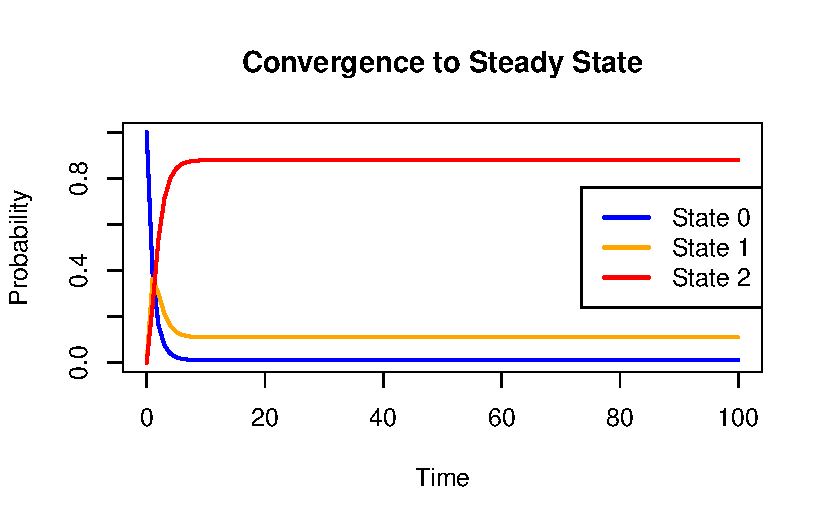
\includegraphics[keepaspectratio]{ctmc_queueing_theory_lab_with_answers_files/figure-pdf/unnamed-chunk-3-1.pdf}}

Explain: How long does it take for the system to reach equilibrium?
Which state dominates during the transient phase?

\emph{\textbf{Answer:}}

\emph{Based on the convergence plot, the system reaches its equilibrium
(steady-state) approximately \textbf{within 15 to 20 minutes}. This is
evident from the point at which the probabilities for all three states
stabilize and no longer change significantly over time.}

\emph{During the \textbf{initial transient phase}, the system starts
from an empty state (State 0), so the probability of being in State 0 is
initially 1. As time progresses, patients begin arriving, and the
probability of being in State 1 (one patient in the room) increases
briefly. However, this is quickly overtaken by State 2 (two patients in
the room), whose probability rises rapidly and becomes the dominant
state.}

\emph{Once equilibrium is reached, \textbf{State 2 clearly dominates},
maintaining a high steady-state probability (approximately 88\%). This
indicates that under the current arrival and observation rates, the
clinic operates at or near full capacity for most of the time.}

\subsection{Task 4. How many people are typically in the
room?}\label{task-4.-how-many-people-are-typically-in-the-room}

On average, how many people are being observed in the room at any given
time? This gives a sense of how often the room is full or idle.

\begin{Shaded}
\begin{Highlighting}[]
\FunctionTok{sum}\NormalTok{(}\DecValTok{0}\SpecialCharTok{:}\DecValTok{2} \SpecialCharTok{*}\NormalTok{ pi)}
\end{Highlighting}
\end{Shaded}

\begin{verbatim}
[1] 1.868132
\end{verbatim}

\subsection{Task 5. What if more patients start coming
in?}\label{task-5.-what-if-more-patients-start-coming-in}

Due to a new outreach campaign and the arrival of a donor-funded vaccine
shipment, community interest in rubella vaccination has surged. As a
result, patients are now arriving every 30 minutes, doubling the
previous arrival rate. Observation lasts 20 minutes when one person is
present. If two patients are present, they both stay for 17 minutes.

How does this change the expected number of patients inside the room?

\begin{Shaded}
\begin{Highlighting}[]
\NormalTok{Q2 }\OtherTok{\textless{}{-}} \FunctionTok{matrix}\NormalTok{(}\FunctionTok{c}\NormalTok{(}
  \SpecialCharTok{{-}}\DecValTok{2}\NormalTok{, }\DecValTok{2}\NormalTok{, }\FloatTok{0.0}\NormalTok{,}
   \DecValTok{1}\SpecialCharTok{/}\DecValTok{20}\NormalTok{, }\SpecialCharTok{{-}}\FloatTok{2.0588}\NormalTok{, }\DecValTok{2}\NormalTok{,}
   \FloatTok{0.0}\NormalTok{, }\DecValTok{1}\SpecialCharTok{/}\DecValTok{17}\NormalTok{, }\SpecialCharTok{{-}}\DecValTok{1}\SpecialCharTok{/}\DecValTok{17}
\NormalTok{), }\AttributeTok{nrow =} \DecValTok{3}\NormalTok{, }\AttributeTok{byrow =} \ConstantTok{TRUE}\NormalTok{)}

\NormalTok{pi2 }\OtherTok{\textless{}{-}} \FunctionTok{steady\_state}\NormalTok{(Q2)}
\FunctionTok{round}\NormalTok{(pi2, }\DecValTok{4}\NormalTok{)}
\end{Highlighting}
\end{Shaded}

\begin{verbatim}
[1] 0.0007 0.0284 0.9709
\end{verbatim}

\begin{Shaded}
\begin{Highlighting}[]
\FunctionTok{sum}\NormalTok{(}\DecValTok{0}\SpecialCharTok{:}\DecValTok{2} \SpecialCharTok{*}\NormalTok{ pi2)  }\CommentTok{\# new expected number}
\end{Highlighting}
\end{Shaded}

\begin{verbatim}
[1] 1.970149
\end{verbatim}

\begin{center}\rule{0.5\linewidth}{0.5pt}\end{center}

\section{Part II: Queueing -- Patient Check-in
Desk}\label{part-ii-queueing-patient-check-in-desk}

In the same rural vaccine clinic, patients begin their visit at a
\textbf{check-in desk} staffed by a single nurse. Patients arrive
randomly, on average once every two minutes. Each check-in takes about
1.5 minutes and is handled one at a time. If the nurse is already
helping someone, the remaining patients wait their turn. There is no
upper limit on how many patients can wait in line.

\subsection{Task 6. How busy is the nurse, and how long do patients
wait?}\label{task-6.-how-busy-is-the-nurse-and-how-long-do-patients-wait}

The clinic administrator wants to know: How busy is the nurse? How long
does each patient spend waiting and checking in? And how many people are
typically in the system?

\begin{Shaded}
\begin{Highlighting}[]
\NormalTok{lambda }\OtherTok{\textless{}{-}} \DecValTok{1}\SpecialCharTok{/}\DecValTok{2}  \CommentTok{\# arrivals per minute}
\NormalTok{mu }\OtherTok{\textless{}{-}} \DecValTok{2}\SpecialCharTok{/}\DecValTok{3}      \CommentTok{\# service rate per minute (1/1.5)}

\NormalTok{rho }\OtherTok{\textless{}{-}}\NormalTok{ lambda }\SpecialCharTok{/}\NormalTok{ mu}
\NormalTok{L }\OtherTok{\textless{}{-}}\NormalTok{ rho }\SpecialCharTok{/}\NormalTok{ (}\DecValTok{1} \SpecialCharTok{{-}}\NormalTok{ rho)}
\NormalTok{Lq }\OtherTok{\textless{}{-}}\NormalTok{ rho}\SpecialCharTok{\^{}}\DecValTok{2} \SpecialCharTok{/}\NormalTok{ (}\DecValTok{1} \SpecialCharTok{{-}}\NormalTok{ rho)}
\NormalTok{W }\OtherTok{\textless{}{-}} \DecValTok{1} \SpecialCharTok{/}\NormalTok{ (mu }\SpecialCharTok{*}\NormalTok{ (}\DecValTok{1} \SpecialCharTok{{-}}\NormalTok{ rho))}
\NormalTok{Wq }\OtherTok{\textless{}{-}}\NormalTok{ rho }\SpecialCharTok{/}\NormalTok{ (mu }\SpecialCharTok{*}\NormalTok{ (}\DecValTok{1} \SpecialCharTok{{-}}\NormalTok{ rho))}

\FunctionTok{list}\NormalTok{(}
  \AttributeTok{Utilization =} \FunctionTok{round}\NormalTok{(rho, }\DecValTok{2}\NormalTok{),}
  \StringTok{"Avg in System (L)"} \OtherTok{=} \FunctionTok{round}\NormalTok{(L, }\DecValTok{2}\NormalTok{),}
  \StringTok{"Avg in Queue (Lq)"} \OtherTok{=} \FunctionTok{round}\NormalTok{(Lq, }\DecValTok{2}\NormalTok{),}
  \StringTok{"Time in System (W)"} \OtherTok{=} \FunctionTok{round}\NormalTok{(W, }\DecValTok{2}\NormalTok{),}
  \StringTok{"Time in Queue (Wq)"} \OtherTok{=} \FunctionTok{round}\NormalTok{(Wq, }\DecValTok{2}\NormalTok{)}
\NormalTok{)}
\end{Highlighting}
\end{Shaded}

\begin{verbatim}
$Utilization
[1] 0.75

$`Avg in System (L)`
[1] 3

$`Avg in Queue (Lq)`
[1] 2.25

$`Time in System (W)`
[1] 6

$`Time in Queue (Wq)`
[1] 4.5
\end{verbatim}

\subsection{Task 7. What happens when more patients keep
coming?}\label{task-7.-what-happens-when-more-patients-keep-coming}

Imagine the clinic gets busier over time --- more patients show up
without any increase in staff. Let's see how the average number of
patients and the uncertainty around that number change.

\begin{Shaded}
\begin{Highlighting}[]
\NormalTok{rho\_vals }\OtherTok{\textless{}{-}} \FunctionTok{seq}\NormalTok{(}\FloatTok{0.01}\NormalTok{, }\FloatTok{0.99}\NormalTok{, }\AttributeTok{by =} \FloatTok{0.01}\NormalTok{)}
\NormalTok{L\_vals }\OtherTok{\textless{}{-}}\NormalTok{ rho\_vals }\SpecialCharTok{/}\NormalTok{ (}\DecValTok{1} \SpecialCharTok{{-}}\NormalTok{ rho\_vals)}
\NormalTok{Var\_vals }\OtherTok{\textless{}{-}}\NormalTok{ rho\_vals }\SpecialCharTok{*}\NormalTok{ (}\DecValTok{1} \SpecialCharTok{+}\NormalTok{ rho\_vals }\SpecialCharTok{{-}}\NormalTok{ rho\_vals}\SpecialCharTok{\^{}}\DecValTok{2}\NormalTok{) }\SpecialCharTok{/}\NormalTok{ (}\DecValTok{1} \SpecialCharTok{{-}}\NormalTok{ rho\_vals)}\SpecialCharTok{\^{}}\DecValTok{2}

\FunctionTok{plot}\NormalTok{(rho\_vals, L\_vals, }\AttributeTok{type =} \StringTok{"l"}\NormalTok{, }\AttributeTok{col =} \StringTok{"red"}\NormalTok{, }\AttributeTok{lwd =} \DecValTok{2}\NormalTok{,}
     \AttributeTok{ylim =} \FunctionTok{c}\NormalTok{(}\DecValTok{0}\NormalTok{, }\DecValTok{40}\NormalTok{), }\AttributeTok{ylab =} \StringTok{"Mean \& Variance in System"}\NormalTok{, }\AttributeTok{xlab =} \StringTok{"Traffic Intensity (ρ)"}\NormalTok{)}
\FunctionTok{lines}\NormalTok{(rho\_vals, Var\_vals, }\AttributeTok{col =} \StringTok{"blue"}\NormalTok{, }\AttributeTok{lwd =} \DecValTok{2}\NormalTok{, }\AttributeTok{lty =} \DecValTok{2}\NormalTok{)}
\FunctionTok{legend}\NormalTok{(}\StringTok{"topleft"}\NormalTok{, }\AttributeTok{legend =} \FunctionTok{c}\NormalTok{(}\StringTok{"Mean"}\NormalTok{, }\StringTok{"Variance"}\NormalTok{), }\AttributeTok{col =} \FunctionTok{c}\NormalTok{(}\StringTok{"red"}\NormalTok{, }\StringTok{"blue"}\NormalTok{), }\AttributeTok{lty =} \FunctionTok{c}\NormalTok{(}\DecValTok{1}\NormalTok{, }\DecValTok{2}\NormalTok{), }\AttributeTok{lwd =} \DecValTok{2}\NormalTok{)}
\end{Highlighting}
\end{Shaded}

\pandocbounded{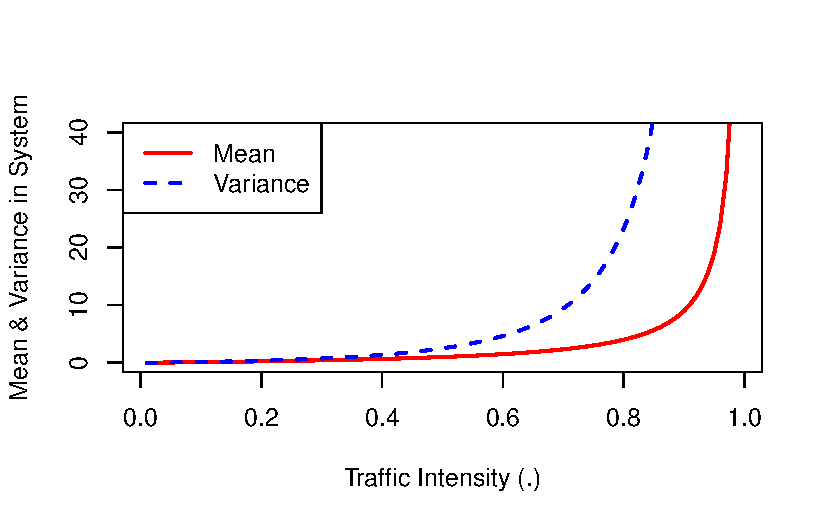
\includegraphics[keepaspectratio]{ctmc_queueing_theory_lab_with_answers_files/figure-pdf/unnamed-chunk-7-1.pdf}}

Explain: What does the graph suggest about the workload and
predictability of the check-in desk as it gets busier?

\textbf{\emph{Answer}}

\emph{As traffic intensity (\(\rho\)) increases, both the \textbf{mean}
and \textbf{variance} of the number of patients in the system grow
rapidly. The red curve in the plot shows the average number of patients
in the system, while the dashed blue curve represents the variance
(i.e., how much the system fluctuates).}

\emph{When the system is lightly loaded (e.g., \(\rho < 0.5\)), both
mean and variance remain low. However, as \(\rho\) approaches 1 ---
meaning patient arrivals nearly match or exceed the nurse's capacity to
serve them --- the average number of people waiting increases sharply,
and the system becomes \textbf{unpredictable}.}

\emph{This pattern suggests that if the clinic continues to get busier
without adding more staff, \textbf{queues will grow longer} and
\textbf{waiting times will become highly variable}, making it hard to
manage patient flow effectively. Clinic managers should aim to keep
traffic intensity well below 1 to ensure smooth and stable operations.}




\end{document}
